\documentclass{article}

\usepackage{url}
\usepackage{a4wide}
\usepackage{color}
\usepackage{eurosym}
\usepackage{hyperref}
\usepackage{multirow}
\usepackage{graphicx}

\pdfpagewidth  200mm
\pdfpageheight 297mm

\addtolength{\oddsidemargin}{-.6in}
\addtolength{\evensidemargin}{-.2in}
\addtolength{\textwidth}{1.4in}
\addtolength{\topmargin}{-.8in}
\addtolength{\textheight}{0.5in}

%avoid figures from occupying the whole page
\renewcommand{\topfraction}{0.95}
\renewcommand{\textfraction}{0.05}
\renewcommand{\floatpagefraction}{0.85}


\newcommand{\hl}[1]{{\large{\sc \underline {#1}}}}

\begin{document}

\section*{Fifth {\sc Pencil Code} User Meeting, Heidelberg, 2009}

\subsection*{Abstract}

The {\sc Pencil Code} User Meeting is an annual meeting dedicated to the Pencil
Code. The purpose of the meeting is to bring regular users and core
developers together to discuss scientific and technical progress since
the last meeting, to instigate collaborative projects and to allow new
users to learn more about the code and to interact with other users
and developers

\subsection*{Scientific summary}

The Pencil
Code\footnote{\url{http://www.nordita.org/software/pencil-code/}} is a
highly versatile and modular code for massively parallel computations. The
project is unique in the astrophysical community in that the code is
continuously developed by a number of independent researchers. The development
is kept in alignment through the use of a version control system (SVN) that
allows the developers to work on different aspects of the code, while still
working within a single branch (Fig.~\ref{fig}, left panel). Automated nightly checks of a large number of
physical standard problems ensures that no new development will break the
code (Fig.~\ref{fig}, right panel).

\begin{figure}[h!]
\center{
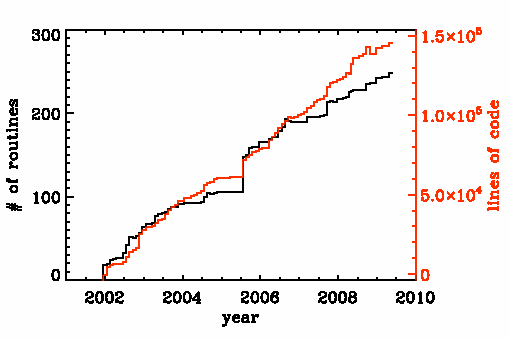
\includegraphics[scale=0.35]{fig/code_size.png}
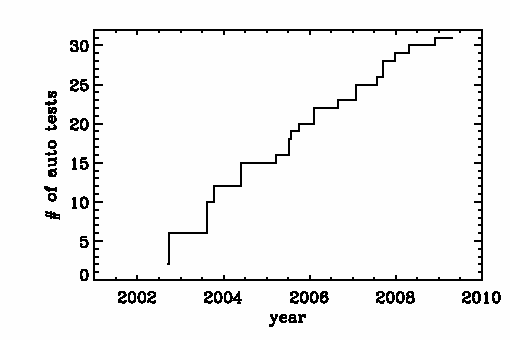
\includegraphics[scale=0.35]{fig/autotests.png}
}
\caption{Left: evolution of the number of routines and lines in
the code since 2002. Right: same for the auto tests checked
every night.}
\label{fig}
\end{figure}

The {\sc Pencil Code} is primarily designed to deal with weakly compressible
turbulent flows, which is why we use high-order spatial derivatives.  To
achieve good parallelization, we use explicit (as opposed to compact) finite
differences. Typical scientific targets include driven MHD turbulence in a
periodic box, convection in a slab with non-periodic upper and lower
boundaries, a convective star embedded in a fully non-periodic box, accretion
disc turbulence in the shearing sheet approximation, planetesimal formation by
self-gravity in turbulent flows, etc. The code is parallelised using the MPI
(Message Passing Interface) library and has been successfully tested on up to
1,000 processors at $1024^3$ grid points, with near linear scaling.
\\ \\
The {\sc Pencil Code} can be downloaded freely from the web-page$^1$, supplying the
astrophysical community with an ideal tool for solving the partial differential
equations of hydrodynamics and magnetohydrodynamics. The {\sc Pencil Code} community
consists of approximately 10-15 main developers and 500 regular users who have
downloaded the code. The code is open source, and we have recently moved the 
repository to Google Code
{\footnote{\url{http://pencil-code.googlecode.com/}}}. 
Registered users can update their copy of the code with the latest version 
through SVN.
\\ \\
The {\sc Pencil Code} User Meeting 2009 will take place August 24-28 2009 at the
Max-Planck Institute for Astronomy, in Heidelberg, Germany. The annual 
{\sc Pencil Code} User Meeting is a workshop
that brings the core developers and regular users together to discuss recent
progress and future challenges related to the {\sc Pencil Code}. Pencil
Code meetings have taken place since 2005 and have proved crucial for keeping
developers aligned about future priorities and for introducing new users to the
code.
\\ \\
Here are some topics that the meeting aims at covering:
\begin{itemize}
  \item Recent science results obtained with the {\sc Pencil Code}
  \item A {\sc Pencil Code} paper
   \item Future improvements to the code
  \item Exchange of experience and ideas
\end{itemize}
The website of the meeting can be found at\\
\url{http://agenda.albanova.se/conferenceDisplay.py?confId=1190}.\\

The webpages of the former {\sc Pencil Code} meetings can be found at the 
following links

\begin{tabular}{ll}
2008& 4th PC meeting, Leiden Observatory (Leiden) \\
    &\url{http://www.strw.leidenuniv.nl/~ajohan/pencil2008/} \\
2007& 3rd PC meeting, NORDITA (Stockholm)\\
    &\url{http://agenda.albanova.se/conferenceDisplay.py?confId=185}\\

2006& 2nd PC meeting, NORDITA (Copenhagen)\\
    &\url{http://www.nordita.dk/conference/PencilCode06/}\\

2005& 1st PC meeting, NORDITA (Copenhagen)\\
    & \url{http://www.nordita.org/~brandenb/get-together/meetings/pencil-workshop05a.html}
\end{tabular}

\subsection*{Provisional list of participants}

Currently 24 people have registred online, 9 of these being local participants (from MPIA). 
For comparison, last year's meeting in 
Leiden{
\footnote{See \url{http://www.strw.leidenuniv.nl/~ajohan/pencil2008/}}} 
had 21 participants. 
The 2007 meeting in Stockholm{
\footnote{See \url{http://agenda.albanova.se/conferenceDisplay.py?confId=185}}} 
had 19. The participant list is shown in Table~\ref{tab:participants}.
\\ 
\begin{table}
\caption[]{Participant list.}
\label{tab:participants}
\begin{center}
  \begin{tabular}{llll}\hline
    Last name & First name & Institution & Country\\
    \hline
    Babkovskaia &  Natalia     &  SINTEF Energy Research & Norway\\
    Bingert     &  Sven        &  Kiepenheuer Institute for Solar Physics & Germany\\
    Brandenburg &  Axel        &  Nordic Institute for Theoretical Physics & Sweden\\
    Candelaresi &  Simon       &  Nordic Institute for Theoretical Physics & Sweden\\
    Clark       &  Dayton      &  Brooklyn College/CUNY & USA\\
    Dintrans    &  Boris       &  Observatoire Midi-Pyr\'en\'ees & France\\
    Dobler      &  Wolfgang    &  Private company & Germany\\
    Dzyukevich  &  Natalia     &  Max-Planck-Institut f\"ur Astronomie & Germany\\
    Flock       &  Mario       &  Max-Planck-Institut f\"ur Astronomie & Germany\\
    Gaburov     &  Evghenii    &  Leiden Observatory & The Netherlands \\
    Haugen      &  Nils        &  SINTEF Energy Research & Norway\\
    Heinemann   &  Tobias      &  DAMPT, Cambridge & UK \\
    Johansen    &  Anders      &  Leiden Observatory & The Netherlands\\
    Kern        &  Sebastian   &  Max-Planck-Institut f\"ur Astronomie & Germany\\
    Klahr       &  Hubert      &  Max-Planck-Institut f\"ur Astronomie & Germany\\
    Kragset     &  Steinar     &  SINTEF Energy Research & Norway\\
    Kuiper      &  Rolf        &  Max-Planck-Institut f\"ur Astronomie & Germany\\
    Lyra        &  Wladimir    &  Max-Planck-Institut f\"ur Astronomie & Germany\\
    Mac Low     &  Mordecai    &  American Museum of Natural History & USA\\
    Mitra       &  Dhrubaditya &  Queen Mary College, London & UK \\
    Raettig     &  Natalie     &  Max-Planck-Institut f\"ur Astronomie & Germany\\
    Sundberg    &  Mikaela     &  Stockholm University & Sweden\\
    Vaidya      &  Bhargav     &  Max-Planck-Institut f\"ur Astronomie & Germany\\
    Zsom        &  Andras      &  Max-Planck-Institut f\"ur Astronomie & Germany\\\hline  
\end{tabular}
\end{center}
\end{table}

\subsection*{Meeting programme}

The preliminary program of the {\sc Pencil Code} User Meeting 2009 is available online at \\

\url{http://agenda.albanova.se/conferenceTimeTable.py?confId=1190}. 

From Monday 
to Thursday the morning sessions will consist of classical talks, meaning speakers 
and slides. As in the previous meetings, there will be both technical and scientific 
talks, with the primary goal of exchange of ideas. The afternoon sessions will see 
discussions of predefined topics. The discussions are led by one or a few
developers, occurring 
in a relaxed and informal way. The issues are usually technical, so the afternoon discussions 
are more palatable for developers and heavy users, but it also constitutes a good 
learning opportunity for newcomers and non-users, in order to understand the 
internals of the code and how it is organized. The feedback of newcomers and non-users 
in the discussion sessions of the previous meetings has also proved vital for the 
developers as well.

On Friday we reserve the day to work on the topics discussed during the meeting - hacking the 
code and fixing bugs. This day is of course optional, and we expect mostly the developers to be 
present. We show the preliminary program in Table~\ref{tab:program}.
\\ 

\begin{table}
\caption[]{Program of the Meeting.}
\label{tab:program}
\begin{center}
\begin{tabular}{|l||cl|}\hline
\multirow{6}{*}{Monday}   &10:00 - 10:30&Dead zones in global models of protoplanetary disks (Lyra)\\
                          &10:30 - 11:00&Particle collisions and particle discs (Johansen)\\
                          &11:30 - 12:00&Science with Pencil at AMNH - Current status (Mac Low)\\
                          &12:00 - 12:30&{\sc Pencil Code} on many core architectures (Clark)\\
                          &14:00 - 16:00&Discussion: Auto-test (Dobler/Brandenburg/Dintrans)\\
                          &16:00 - 18:00&Discussion: Anelastic solver (Dintrans)\\\hline
%
\multirow{6}{*}{Tuesday}  &10:00 - 10:30&MHD simulations of the solar corona (Bingert)\\
                          &10:30 - 11:00&The new configuration scheme (Dobler)\\
                          &11:30 - 12:00&Fargo vs Pencil - A comparison study (Zsom)\\
                          &12:00 - 12:30&The Pluto code (Flock)\\
                          &14:00 - 16:00&Discussion: Configuration (Dobler/Brandenburg)\\
                          &16:00 - 18:00&Discussion: Initial conditions (Johansen)\\\hline
%
\multirow{6}{*}{Wednesday}&10:00 - 10:30&Star-in-a-box simulations of solar-like dynamos (Dintrans)\\
                          &10:30 - 11:00&Non-conservative Lagrangian + conservative remap scheme (Gaburov)\\
                          &11:30 - 12:00&Current status of the combustion module (Babkovskaia)\\
                          &12:00 - 12:30&MHD dynamos in spherical wedges : recent results (Mitra)\\
                          &14:00 - 16:00&Discussion: Polar coordinates (Lyra/Mitra/Dintrans)\\
                          &16:00 - 18:00&Discussion: Bug list / Miscellaneous\\\hline
%
\multirow{6}{*}{Thursday} &10:00 - 10:30&Particle deposition on a cylinder in a cross flow (Haugen)\\
                          &10:30 - 11:00&Solid geometries with the immersed boundary method (Kragset)\\
                          &11:30 - 12:00&Lightsabers with the {\sc Pencil Code} (Brandenburg)\\
                          &12:00 - 12:30&Organizing simulation code collectives (Sundberg)\\
                          &14:00 - 16:00&Discussion: Nested Pencil / Pencil AMR (Johansen/Lyra)\\
                          &16:00 - 18:00&Discussion: Bug list / Miscellaneous\\\hline
\end{tabular}
\end{center}
\end{table}

\subsection*{Budget}

Of the 15 non-local participants, 10 will eligible for travel
support, based on their junior positions (PhD students, young
postdocs) or on positions in institutions that are not able to provide
travel support. Lunch and coffee would be provided for every participant,
independently of whether they receive travel support. A conference dinner
should also be included, for all participants.
\\ \\
The estimated costs are (in Euro):
\begin{center}
  \begin{tabular}{|l | r l c c c c c r|}\hline
                & Amount &(& persons &$\times$& days &$\times$& cost &)\\\hline
  Travel        & 3\,000 &(& 10      &$\times$&  1   &$\times$& 300  &)\\
  Accomodation  & 4\,000 &(& 10      &$\times$&  5   &$\times$&  80  &)\\
  Dinner        & 1\,000 &(& 25      &$\times$&  1   &$\times$&  40  &)\\
  Lunch         & 1\,000 &(& 25      &$\times$&  5   &$\times$&   8  &)\\
  Coffee        &    500 &(& 25      &$\times$&  5   &$\times$&   4  &)\\\hline
  \end{tabular}
\end{center}

The total cost is therefore of 9\,500 euros. We herewith
apply for 50\% of this sum, 4\,750 euros. Additional funding request 
will be submitted to the European Science Foundation. MPIA has 
kindly offered a conference room free of charge. 

\clearpage
\newpage

\subsection*{Curriculum vitae of scientific organiser}

\vspace{1cm}

\hl{General Information}

\vspace{2mm}

\begin{tabular}{ll}
  \textbf{Name}: & Wladimir Lyra \\
  \textbf{Current position}: & Postdoctoral fellow at the Max-Plack Institute for Astronomy\\
  \textbf{Birth date}: & 14 December 1981 \\
  \textbf{City of birth}: & Rio de Janeiro \\
  \textbf{Nationality}: & Brazilian \\
  \textbf{Address}: & K\"onigstuhl 17, D-61179, Heidelberg, Germany \\
  \textbf{E-mail}: & \url{wlyra@mpia.de} \\
  \textbf{Telephone number}: &
   (+49) 6221 528 258 (office) / (+49) 176 8530 2225 (mobile) \\
  \textbf{Website}: & \url{http://www.mpia.de/homes/lyra}
\end{tabular}

\vspace{5mm}

\hspace{-.55cm}\hl{Education}

\begin{itemize}

\item{{\bf Ph.D.}

Duration: September 2004 - March 2009 \\
Uppsala University  - Department of Physics and Astronomy

Licentiate (Ph.Lic.) thesis title: \\
{\bf Magnetohydrodynamics of turbulent accretion disks and planet formation }\\
Defended: 31 Oct 2007 (public defense)

Doctoral thesis title: \\
{\bf Turbulence-assisted planetary growth}\\
Defended: 26 Feb 2009 (public defense)}

\item{{\bf B.Sc.}

Duration: March 1999 - July 2003 \\
Federal University of Rio de Janeiro - Observat{\'o}rio do Valongo\\
Major: Astronomy

Senior thesis title:\\ 
{\bf Calibration of the H$\alpha$ line as chromospheric diagnostic and indicator of age in solar type stars}\\
Defended: 23 July 2003 (public defense)}

\item{{\bf Honors and Awards}

\begin{itemize}

\item{Undergraduate {\it Diploma cum Laude} awarded for graduating with high GPA (9.0/10.0)}
\item{Nomination for {\it Best Senior Thesis} among all hard sciences students from Federal University of Rio de Janeiro}
\item{Nomination for {\it Academic Distinction of 2004} at Federal University of Rio de Janeiro} 
\item{Recipient of the following grants:}
  \begin{itemize}
    \item{CNPq - Conselho Nacional de Desenvolvimento Cient{\'\i}fico e Tecnol{\'o}gico\\
    (National Counsel of Technological and Scientific Development)\\ 
    3000 BRR/year from October 2000 to June 2003}
    \item{Anna and Allan L\"ofbergs stipend 14\,0000 SEK/year from Oct 2004 to Dec 2006}
    \item{Liljewalchs travel stipend. 10\,000 SEK (August 2007)}  
    \item{H{\aa}kansson travel stipend. 35\,000 SEK (June 2008)}  
  \end{itemize}
\end{itemize}}


\item{{\bf Computer experience}

\begin{itemize}
  \item{Operating system: Linux/Unix}
  \item{Programming proficiency:}
    \begin{itemize}
     \item{fluent: Fortran 90, IDL, HTML, IRAF, Supermongo, Linux/C-shell}
     \item{intermediate: Awk, C}
     \item{beginner: Python, Java}
    \end{itemize}
  \item{Webmaster for the Division of Astronomy and Space Physics at Uppsala University during 2005 and 2006}
  \item{Co-developer of the {\sc Pencil Code} (a high-order MPI code for MHD turbulence) since 2005.} 
\end{itemize}}

\item{{\bf Language Proficiency:} 

\begin{itemize}
  \item{Portuguese (native language)}
  \item{English, Spanish (fluent)}
  \item{Swedish (good)}  
  \item{French, Italian, Danish, Norwegian (basic)}  
\end{itemize}}

\end{itemize}

\vspace{5mm}

\hspace{-.55cm}\hl{Employment:}

\begin{itemize}

  \item{
      {\bf {Max-Planck Institute for Astronomy}}\\
      K\"onigstuhl 17, D-61179, Heidelberg, Germany.\\
      Position: Postdoctoral fellow\\
      From-To: Apr 2009 - Oct 2009}

  \item{
      {\bf {Cerro Tololo Interamerican Observatory}}\\
      Casilla 603, La Serena, Chile. \\
      Supervision of: Dr. Nicole S. van der Bliek \\
      Position: Research Assistant\\   
      From-To: Jul 2003 - Jul 2004

      The position at CTIO included visiting trips to:
      \begin{itemize}
      \item{{\bf {European Southern Observatory}}\\
      Karl Schwarzchild Str 2, D-85748 Garching, Germany.\\
      Supervision of: Dr. Jo\~ao Alves \\
      From-To: Aug - Oct 2003}

  \item{{\bf {Lisbon Observatory}}\\
      Tapada da Ajuda, 1349-018, Lisbon, Portugal.\\
      Supervision of: Dr. Andre Moitinho\\ 
      From-To: Sep 2003}
    \end{itemize}

  \item{{\bf  {Space Telescope Science Institute}}\\
      San Martin Drive 3700. Baltimore, MD. USA. \\
      Supervision of: Dr. Daniela Calzetti \\
      Position: Summer Student\\
      From-To: Jun - Sep 2002}
  }

\end{itemize}


\hspace{-.55cm}\hl{Teaching Experience}

\begin{itemize}

\item{{\bf pH High-School and Pre-University Course}\\
    Teaching and tutoring Mathematics and Physics in the preparatory course for admission to University (from February 1999 to September 2000)}

\item{{\bf Federal University of Rio de Janeiro}\\
    Informal Tutoring for Astronomy Students in
    \begin{itemize}
     \item{Statistics (Spring 2001)}
     \item{Electromagnetism (Autumn \& Spring 2002)} 
     \item{Quantum Mechanics (Autumn 2003)}
    \end{itemize}}

\item{{\bf Uppsala University}\\
    Teaching Assistantship for the following courses
    \begin{itemize}
    \item{Physics of the interstellar medium (Autumn 2007)}
    \item{Stellar Physics (Autumn 2007)}
    \item{Classical Mechanics (Autumn 2008)}  
    \end{itemize}}
\end{itemize}

\vspace{5mm}

\hspace{-.55cm}\hl{Advising}

\vspace{5mm}

During my Ph.D. I have advised or co-advised three studies that led to Bachelors Theses at the Department of Physics and Astronomy. These are:
\begin{itemize}
\item{{\bf Radiative transfer in hydrodynamical models of protoplanetary disks}\\
Student: Heidar Thor Thrastarson, 2007}

\item{{\bf Feasibility study of observing planetary perturbations in protoplanetary disks using MIDI at VLTI}\\
Student: Peter Schmidt, Year: 2006}

\item{{\bf Photometric Properties of Metal Poor Stars}\\
Students: Anders Eriksson and Anna \"Onehag, 2005}

\end{itemize}

\vspace{5mm}

\hspace{-.55cm}\hl{Observational Experience}

\begin{itemize}
  \item{{\bf Observat{\'o}rio do Pico dos Dias}\\
      Laborat{\'o}rio Nacional de Astrof{\'\i}sica, Brazil\\
      Extensive experience using the 1.60m telescope at OPD/LNA, performing spectroscopic observations in optical wavelengths with a coude spectrograph. The dates when the observations took place were may/00, oct/00, jun/01, sep/01, oct/01, may/02, oct/02, dec/02.}

    \item{{\bf Cerro Tololo Interamerican Observatory}\\
Seventeen engineering nights at the 4m telescope scattered from oct/03 to jun/04 doing photometric observations of standard stars on JHK wavebands, to test Tololo's new infrared camera, ISPI. Observations were performed under supervision of CTIO staff Dr. Nicole S. van der Bliek and Dr. Dara Norman.}

\end{itemize}

\hspace{-.55cm}\hl{Workshop organization}

\begin{itemize}
    
\item{``{\sc Pencil Code} User Meeting 2009'' - Heidelberg, August 2009. Main organizer}

\item{``Turbulence-Assisted Planetary Growth'' - Uppsala, February 2009. Main organizer}

\item{``Nobel Symposium 135: Physics of Planetary Systems'' - Stockholm, June 2007. Co-organizer}

\end{itemize} 

\vspace{5mm}

\hspace{-.55cm}\hl{Five most relevant scientific publications}

\begin{itemize}
    
\item{Planet formation bursts at the borders of the dead zone in 2D simulations of circumstellar disks\\
\underline{W. Lyra}, A. Johansen, A. Zsom, H. Klahr, \& N. Piskunov 2009, A\&A, 497, 869}

\item{Standing on the shoulders of giants: Trojan Earths and vortex trapping in low-mass self-gravitating protoplanetary disks of gas and solids\\
\underline{W. Lyra}, A. Johansen, H. Klahr, \& N. Piskunov 2009, A\&A, 493, 1125\\
Cover image of A\&A vol. 493}

\item{Embyros grown in the dead zone: Assembling the first protoplanetary cores in low-mass self-gravitating circumstellar disks of gas and solids\\
\underline{W. Lyra}, A. Johansen, H. Klahr, \& N. Piskunov 2008, A\&A, 491L, 41\\
Highlighted letter at A\&A vol. 491}

\item{Global magnetohydrodynamical models of turbulence in protoplanetary disks\\
I. A cylindrical potential on a Cartesian grid and transport of solids\\
\underline{W. Lyra}, A. Johansen, H. Klahr, \& N. Piskunov 2008, A\&A, 479, 883.}

\item{On the difference between nuclear and contraction ages\\
\underline{W. Lyra}, A. Moitinho, N. S. van der Bliek, \& J. Alves 2006 A\&A, 453, 101.}

\end{itemize} 


\end{document}
